\section{System overview}
Our robots hardware does not change much since Robocup Asia-Pacific in 2017 which consist of 5 robots comprised of 2 sizes; 3 with 57 cm tall, and 2 with 47 cm as shown in Fig \ref{fig:humanoid}. Each robot have mechanical hardware, sensors, computing hardware and 20 Dynamixel servo-motor. The structure of all robots is made of aluminum alloy sheet metal(details are provided in the robot specification sheet).
\begin{figure}[H]
	\centering
	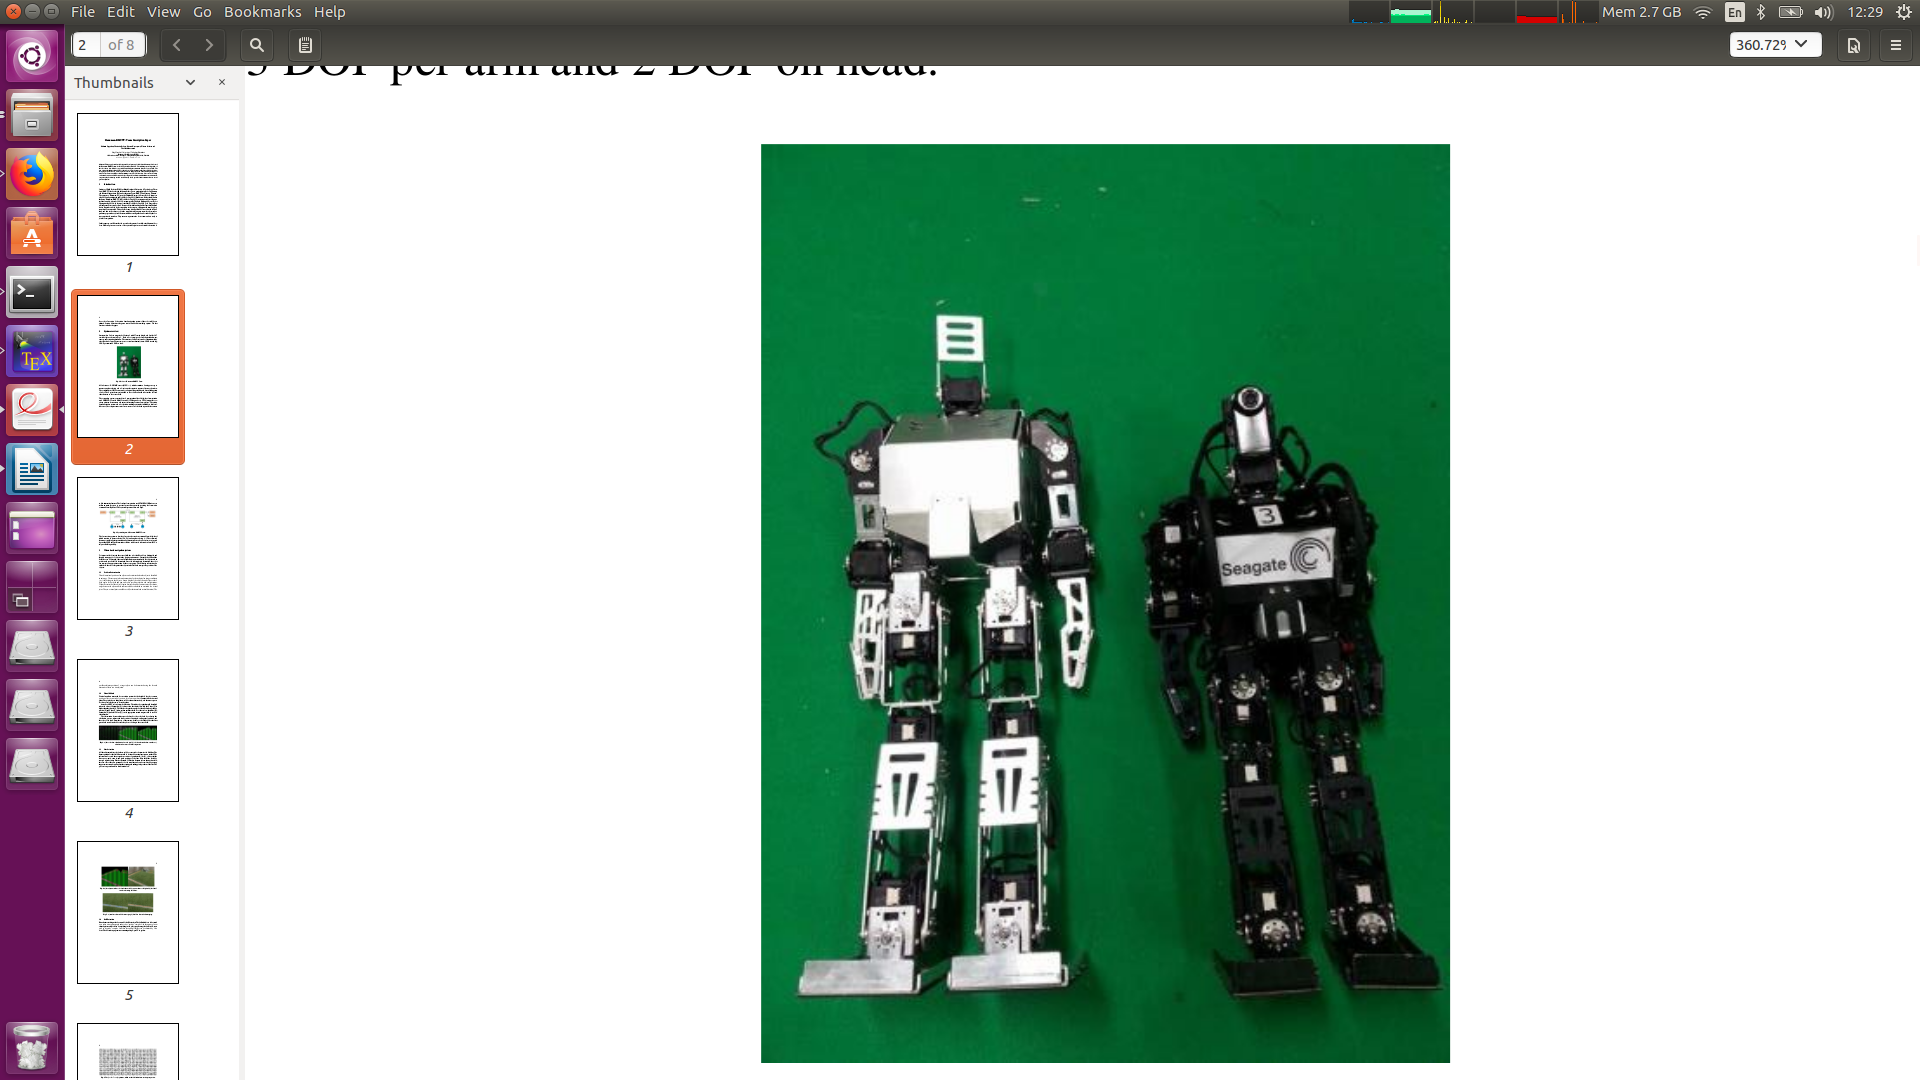
\includegraphics[width=\textwidth,trim={15cm 0cm 5cm 5cm},clip]{image/humanoid.png}
	\caption{Robots of Hanuman-KMUTT Team}
	\label{fig:humanoid}
\end{figure}
All robots use 6 DOF IMU sensor (MPU- 6500 ) which contains a 3-axis gyroscope and a 3-axis accelerometer. The combination of IMU sensor used to adapt walking stability and detect falling state of robot. The Logitech camera installed. The computing system consist of 2 separate systems; high-level and low-level as we described in \cite{TDP:Nakarin}. High-level computation used DROID-C1+ with ARM Cortex-A5 (1.5Ghz quad core CPUs) for computing image processing, decision making and navigation. Low-level computation used STM32F411RE micro-controller for operating locomotion system.
\begin{figure}[H]
	\centering
	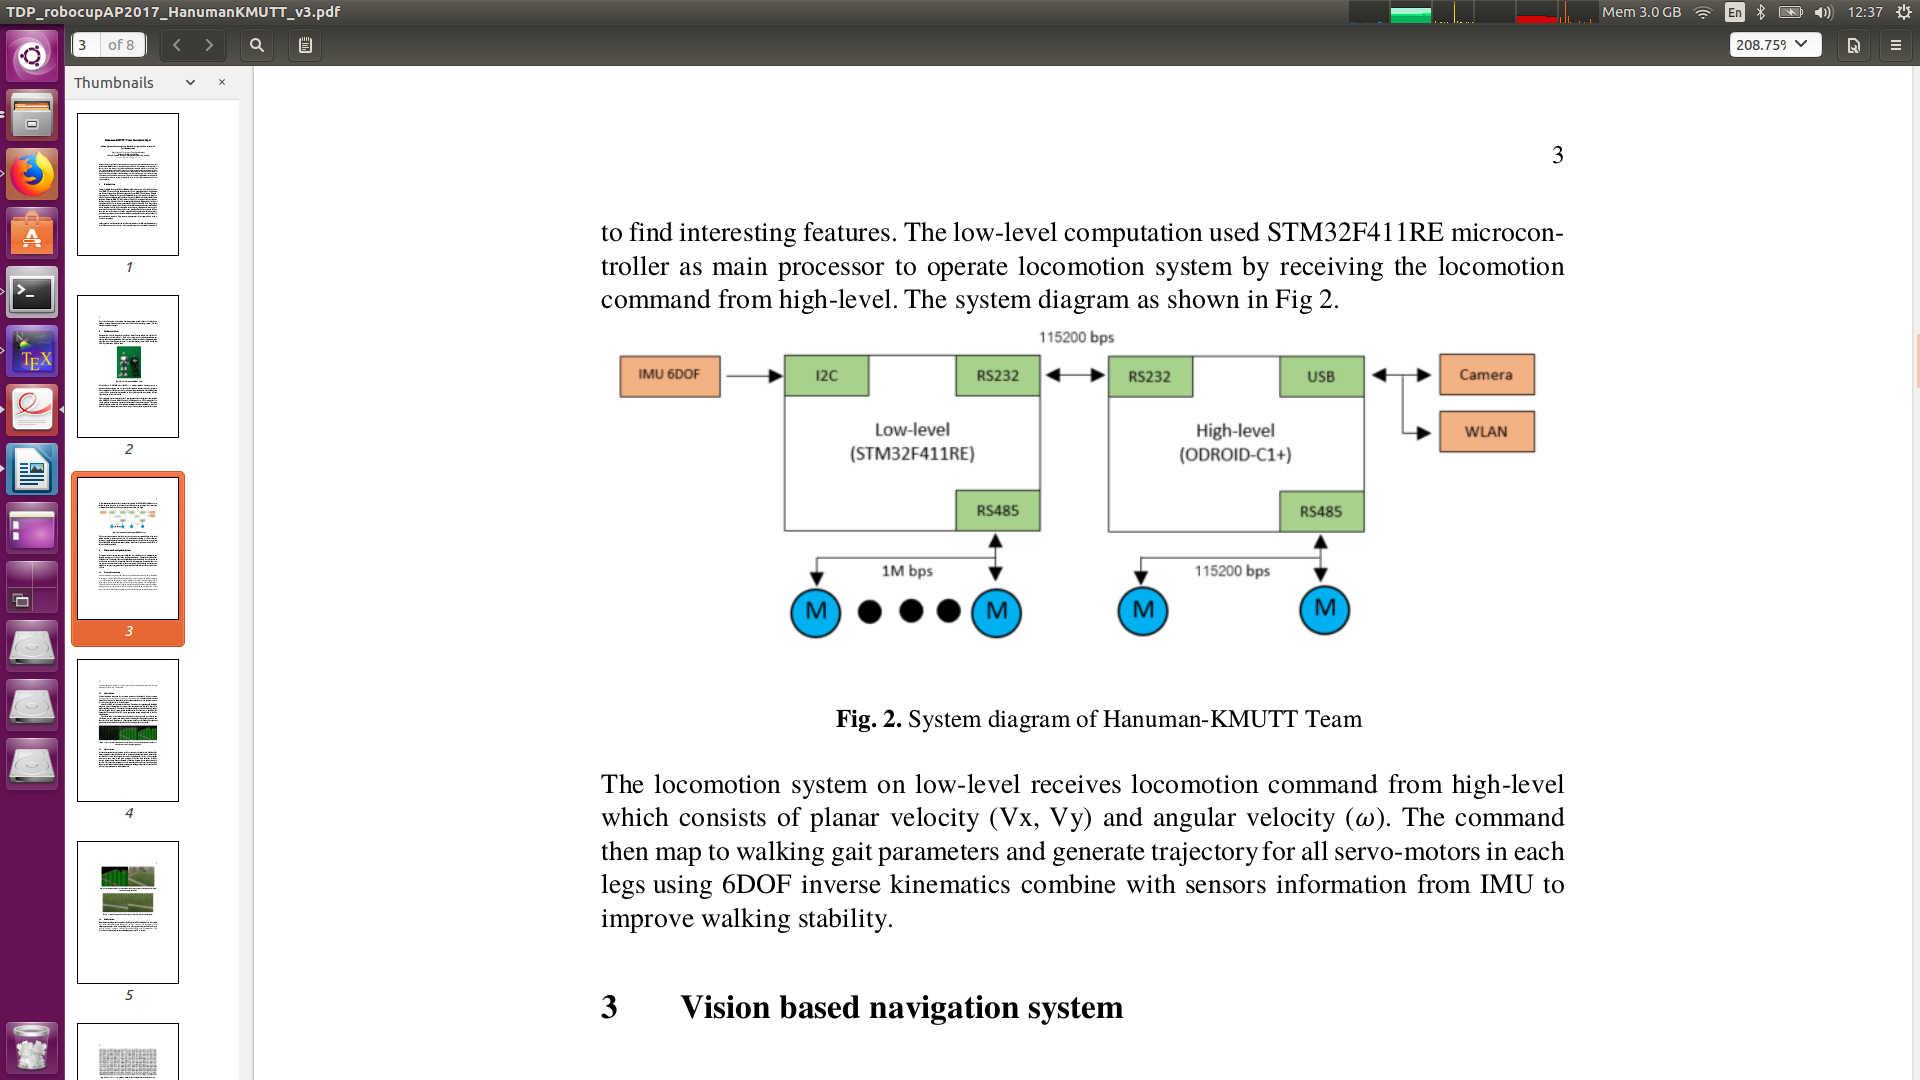
\includegraphics[width=\textwidth,trim={20cm 15cm 10cm 12.5cm},clip]{image/sysDiagram.png}
	\caption{System diagram of the computing system in the Hanuman-KMUTT Team}
	\label{fig:sysDiagram}
\end{figure}